

\begin{figure}[htbp]
    \centering
    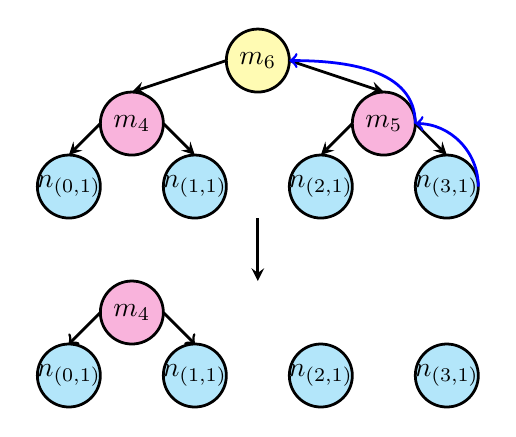
\begin{tikzpicture}[scale=0.4] % Adjust the scale factor as needed
        % Your TikZ code goes here
        \draw[line width=1pt,fill=yellow!30] (0,0) circle (1cm);
        \node at (0,0) {$m_6$};
        \draw[line width=1pt, fill=magenta!30] (-4,-2) circle (1cm);
        \node at (-4,-2) {$m_4$};
        \draw[line width=1pt, fill=magenta!30] (4,-2) circle (1cm);
        \node at (4,-2) {$m_5$};
        \draw[line width=1pt, fill=cyan!30] (-6,-4) circle (1cm);
        \node at (-6,-4) {$n_{(0,1)}$};
        \draw[line width=1pt, fill=cyan!30] (-2,-4) circle (1cm);
        \node at (-2,-4) {$n_{(1,1)}$};
        \draw[line width=1pt, fill=cyan!30] (6,-4) circle (1cm);
        \node at (6,-4) {$n_{(3,1)}$};
        \draw[line width=1pt, fill=cyan!30] (2,-4) circle (1cm);
        \node at (2,-4) {$n_{(2,1)}$};
        \draw[-> , >=stealth,line width=1pt] ({0 + cos(180)},{0 + sin(180)}) -- (-4,-1);
        \draw[->, >=stealth, line width=1pt] ({0 + cos(0)},{0 + sin(0)}) -- (4,-1);
        \draw[->, >=stealth, line width=1pt] ({-4 + cos(180)},{-2 + sin(180)}) -- (-6,-3);
        \draw[->, >=stealth, line width=1pt] ({-4 + cos(0)},{-2 + sin(0)}) -- (-2,-3);
        \draw[->, >=stealth, line width=1pt] ({4 + cos(180)},{-2 + sin(180)}) -- (2,-3);
        \draw[->, >=stealth, line width=1pt] ({4 + cos(0)},{-2 + sin(0)}) -- (6,-3);
        
        % Curved arrow
        \draw[->, color=blue, line width=1pt] (7, -4) to[out=90, in=0] (5, -2);
        \draw[->, color=blue, line width=1pt] (5, -2) to[out=90, in=0] (1, 0);
        \draw[->, >=stealth, line width=1pt] (0,-5) to (0,-7);

        \draw[line width=1pt, fill=magenta!30] (-4,-8) circle (1cm);
        \node at (-4,-8) {$m_4$};
        \draw[line width=1pt, fill=cyan!30] (-6,-10) circle (1cm);
        \node at (-6,-10) {$n_{(0,1)}$};
        \draw[line width=1pt, fill=cyan!30] (-2,-10) circle (1cm);
        \node at (-2,-10) {$n_{(1,1)}$};
        \draw[line width=1pt, fill=cyan!30] (6,-10) circle (1cm);
        \node at (6,-10) {$n_{(3,1)}$};
        \draw[line width=1pt, fill=cyan!30] (2,-10) circle (1cm);
        \node at (2,-10) {$n_{(2,1)}$};
    
        \draw[->, line width=1pt] ({-4 + cos(180)},{-8 + sin(180)}) -- (-6,-9);
        \draw[->, line width=1pt] ({-4 + cos(0)},{-8 + sin(0)}) -- (-2,-9);

    \end{tikzpicture}
    \caption{Trees and Cuts}
    \label{fig:Order_of_merging}
\end{figure}
